\begin{figure}
  \centering
  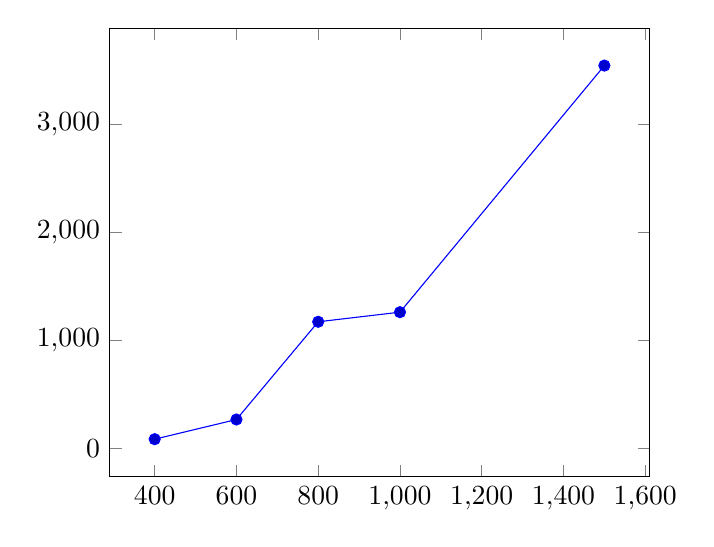
\begin{tikzpicture}
    \begin{axis}
      \addplot coordinates{ % Timing
       (400, 85.1)
       (600, 267.4)
       (800, 1172.9)
       (1000, 1261.9)
       (1500, 3546.5)
      };
    \end{axis}
  \end{tikzpicture}
  \caption{Results for the stage decomposition algorithm: Run times in seconds over the number of scenarios of the initial distribution. At 2000 scenarios, the algorithm failed on 4GB RAM due to memory problems.}
  \label{fig:naive-milp-results-timing}
\end{figure}
\begin{figure}
  \centering
  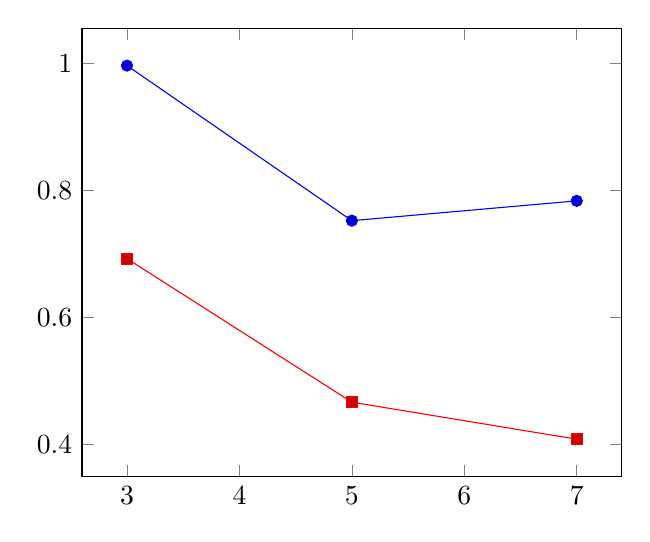
\begin{tikzpicture}
    \begin{axis}%[error bars/y explicit] 
      \addplot  coordinates { % random selection (ultra-naive algorithm)
        (3, 0.9967) %+ (0,0.2379) - (0,0.1479)
        (5, 0.7525) %+ (0,0.1338) - (0,0.0830)
        (7, 0.7837) %+ (0,0.1562) - (0,0.0697)
      };
      \addplot coordinates { % stage-wise MILP
        (3, 0.6927)
        (5, 0.4667)
        (7, 0.4084)
      };
    \end{axis}
    \end{tikzpicture}
  \caption{Results for the stage decomposition algorithm using an MILP solver for each stage for different numbers of children/branches. Number of stages: $n_s=3$, distribution: log-normal, initial value 1, $\mu=0,\,\sigma=0.5$}
  \label{fig:naive-milp-results-errors}
\end{figure}
%%% Local Variables: 
%%% mode: latex
%%% TeX-master: "da"
%%% End: 
